\documentclass[usenames,dvipsnames,9pt]{beamer}
\usetheme[block=fill]{ru}           % Use ru theme

\usepackage{xpatch}
\usepackage{textcomp}
\newcommand{\textapprox}{\raisebox{0.5ex}{\texttildelow}}
\usepackage{listings}
\usepackage{realboxes}

\definecolor{mygray}{rgb}{0.9,0.9,0.9}
\lstset{%
basicstyle=\ttfamily,
breaklines = true,
backgroundcolor=\color{mygray},
}

\makeatletter
\xpretocmd\lstinline{\Colorbox{mygray}\bgroup\appto\lst@DeInit{\egroup}}{}{}
\makeatother

\title{Advanced Use of Git}

\author[Viguier]
{Beno\^{i}t Viguier}

\date[Short Occasion]{\vspace{0.5cm}DS-Lunch Talk,\\Nijmegen, October 25th, 2019}

\begin{document}

% -------------------------------------------------------------
%
% -------------------------------------------------------------
\begin{frame}
  \titlepage
\end{frame}

% -------------------------------------------------------------

% -------------------------------------------------------------
\begin{frame}{Disclaimer}
  \begin{center}
    \alert{\Large{\textbf{If you don't like command line interface,\\this talk is not for you.}}}
  \end{center}
\end{frame}

% -------------------------------------------------------------
%
% -------------------------------------------------------------
\begin{frame}{Minimal Git Commands}
  \begin{itemize}
    \item \lstinline|git clone git@gitlab.science.ru.nl:user/repo|
    \item \lstinline|git status|
    \item \lstinline|git add <directory/files>|
    \item \lstinline|git commit|
    \item \lstinline|git push|
    \item \lstinline|git pull|
  \end{itemize}
\end{frame}

% -------------------------------------------------------------
%
% -------------------------------------------------------------
\begin{frame}{Git Status}
  \begin{itemize}
    \item \lstinline|git status|
    \item \lstinline|git log|
  \end{itemize}

  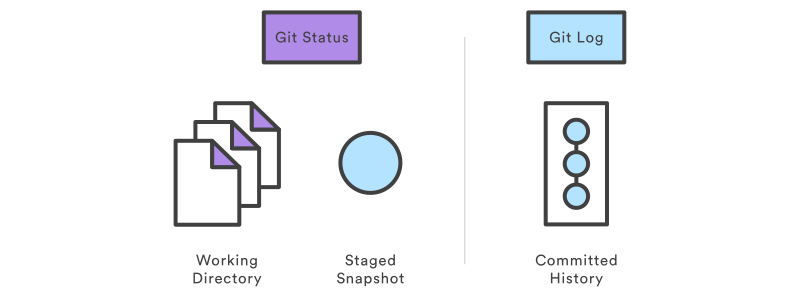
\includegraphics[width=0.8\textwidth]{img/inspecting/01.png}
\end{frame}

% -------------------------------------------------------------
%
% -------------------------------------------------------------
\begin{frame}{Shortcuts}
  \begin{itemize}
    \item \lstinline|git add --all| \hspace{1cm}(\lstinline|-A|)\\
    \emph{Add all the updated/untracked files.}
    \item \lstinline|git add --update| \hspace{1cm}(\lstinline|-u|)\\
    \emph{Add all the updated files but do not add the untracked ones.}
    \item \lstinline|git add --patch| \hspace{1cm}(\lstinline|-p|)\\
    \emph{Similar to update. Interactively lets you decide which modifications in each file you want to save.}
    \item \lstinline|git commit -m "commit message"|
  \end{itemize}
\end{frame}



%%%%%%%%%%%%%%%%%%%%%%%%%%%%%%%%%%%%%%%%%%%%%%%%%%%%%%%
%
%          Branches
%
%%%%%%%%%%%%%%%%%%%%%%%%%%%%%%%%%%%%%%%%%%%%%%%%%%%%%%%
\section{branches}

% -------------------------------------------------------------
%
% -------------------------------------------------------------
\begin{frame}{Branches}
  \begin{itemize}
    \item Develop features without breaking master.\\
    $\implies$ the master branch always compiles! {\color{OliveGreen}\checkmark}
    \item Develop multiple features at the same time.
  \end{itemize}
  \vspace{0.5cm}
  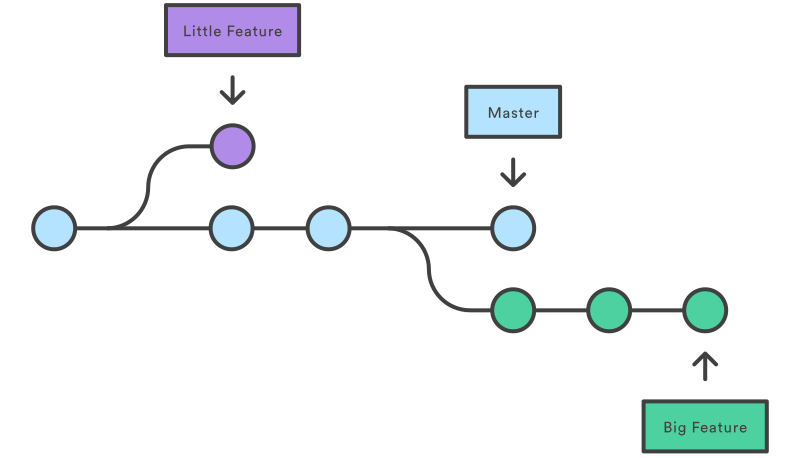
\includegraphics[width=0.8\textwidth]{img/branches/01.png}
\end{frame}

% -------------------------------------------------------------
%
% -------------------------------------------------------------
\begin{frame}{Branches}
  \vspace{-0.45cm}
  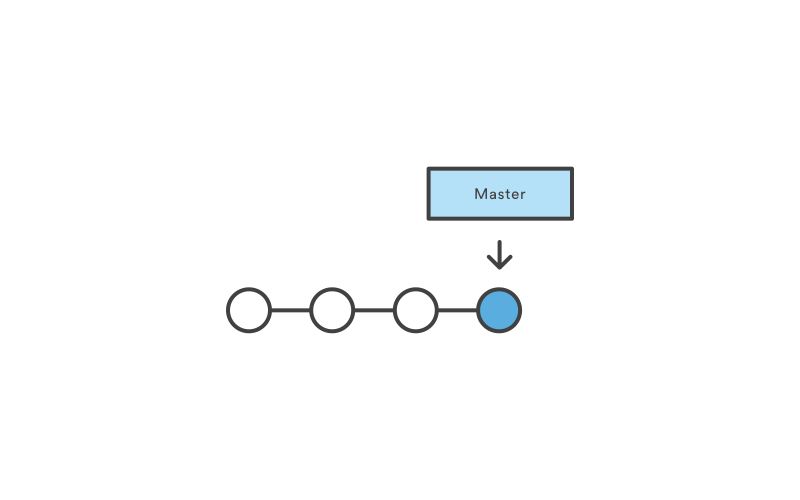
\includegraphics[width=0.8\textwidth]{img/branches/02.png}
\end{frame}

% -------------------------------------------------------------
%
% -------------------------------------------------------------
\begin{frame}{Branches}
  \begin{itemize}
    \item Create a branch \lstinline|git branch Future-plans|
    \item Switch to that branch \lstinline|git checkout Future-plans|
  \end{itemize}
  \vspace{-1cm}
  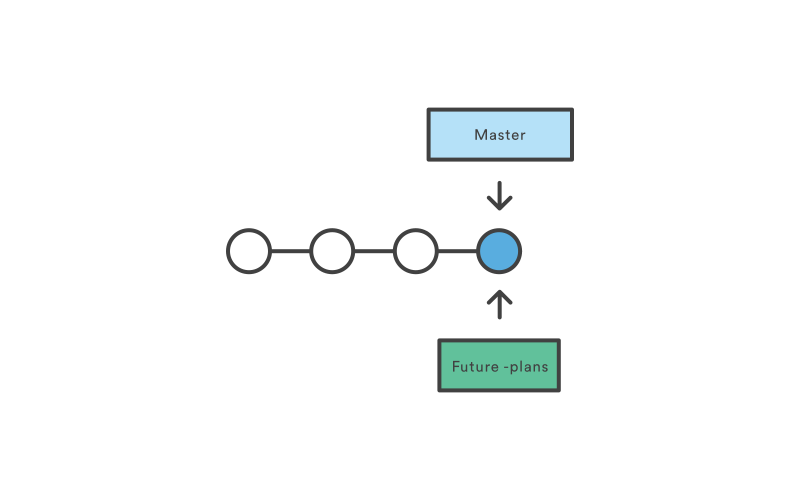
\includegraphics[width=0.8\textwidth]{img/branches/03.png}
  \vspace{-1cm}

  These two can be done in one step: \lstinline|git checkout -b Future-plans|
\end{frame}

% -------------------------------------------------------------
%
% -------------------------------------------------------------
\begin{frame}{Branches}
  Work (modify, commits\ldots) on the \texttt{Future-plans}.\\
  In the meantime, the \texttt{Master} branch continues forward (other commits\ldots)
  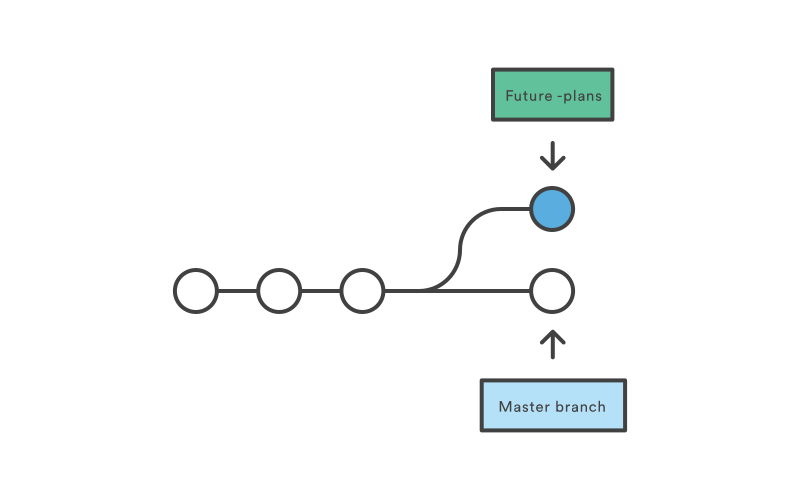
\includegraphics[width=0.8\textwidth]{img/branches/04.png}
\end{frame}

% -------------------------------------------------------------
%
% -------------------------------------------------------------
\begin{frame}{Branches}
  If nothing was done on \texttt{Master} while you were working on \texttt{Future-plans} you can directly merge. This is called \emph{fast-forward}.
  \begin{enumerate}
    \item Switch to the master branch: \lstinline|git checkout master|
    \item Merge: \lstinline|git merge Future-plans|
  \end{enumerate}
  \vspace{-1cm}
  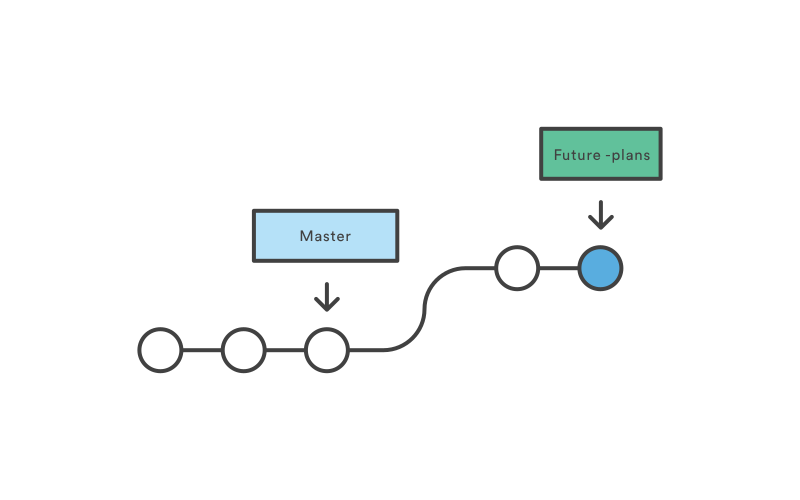
\includegraphics[width=0.8\textwidth]{img/branches/05.png}
\end{frame}

% -------------------------------------------------------------
%
% -------------------------------------------------------------
\begin{frame}{Branches}
  \vspace{0.2cm}
  If nothing was done on \texttt{Master} while you were working on \texttt{Future-plans} you can directly merge. This is called \emph{fast-forward}.
  \begin{enumerate}
    \item Switch to the master branch: \lstinline|git checkout master|
    \item Merge: \lstinline|git merge Future-plans|
  \end{enumerate}
  \vspace{-0.8cm}
  \hspace{0.07cm}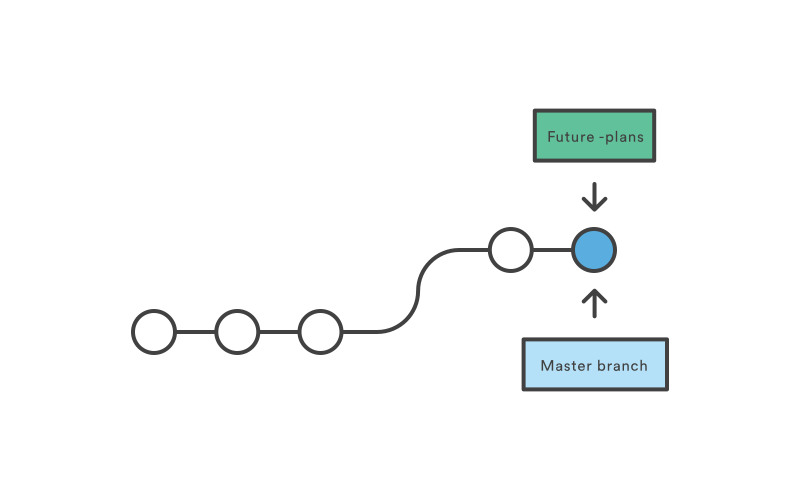
\includegraphics[width=0.8\textwidth]{img/branches/06.png}
\end{frame}

% -------------------------------------------------------------
%
% -------------------------------------------------------------
\begin{frame}{Branches}
  \centering
  To push/update a branch on the online repository:\\
  \lstinline|git push origin Future-plans|\\
  \vspace{1cm}
  To delete (\lstinline|-d|) a branch on the online repository:\\
  \lstinline|git push -d origin Future-plans|\\
  \vspace{1cm}
  To delete (\lstinline|-D|) locally a branch:\\
  \lstinline|git branch -D <branch-name>|\\
  (Not possible while you are on that branch.)
\end{frame}



%%%%%%%%%%%%%%%%%%%%%%%%%%%%%%%%%%%%%%%%%%%%%%%%%%%%%%%
%
%          Merging
%
%%%%%%%%%%%%%%%%%%%%%%%%%%%%%%%%%%%%%%%%%%%%%%%%%%%%%%%
\section{Merging}

% -------------------------------------------------------------
%
% -------------------------------------------------------------
\begin{frame}{Merging}
  If \texttt{Master} has changed while you were working on \texttt{Future-plans} the merge process is slightly different.
  \begin{enumerate}
    \item Switch to the master branch: \lstinline|git checkout master|
    \item Merge: \lstinline|git merge Future-plans|
    \item Edit the commit message in your editor, save and close.
  \end{enumerate}
  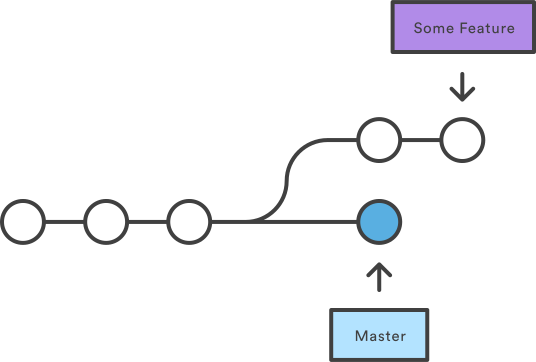
\includegraphics[width=0.608\textwidth]{img/merge/08.png}
\end{frame}

% -------------------------------------------------------------
%
% -------------------------------------------------------------
\begin{frame}{Merging}
  \texttt{Master} has changed while you were working on \texttt{Future-plans} the merge process is slightly different.
  \begin{enumerate}
    \item Switch to the master branch: \lstinline|git checkout master|
    \item Merge: \lstinline|git merge Future-plans|
    \item Edit the commit message in your editor, save and close.
  \end{enumerate}
  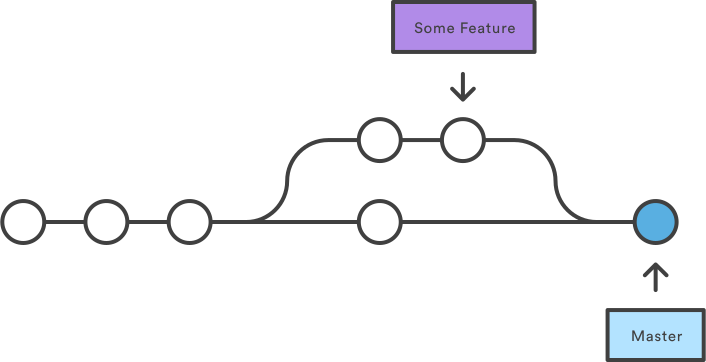
\includegraphics[width=0.8\textwidth]{img/merge/09.png}
\end{frame}



%%%%%%%%%%%%%%%%%%%%%%%%%%%%%%%%%%%%%%%%%%%%%%%%%%%%%%%
%
%          Rebase
%
%%%%%%%%%%%%%%%%%%%%%%%%%%%%%%%%%%%%%%%%%%%%%%%%%%%%%%%
\section{Rebasing}

% -------------------------------------------------------------
%
% -------------------------------------------------------------
\begin{frame}{Merging \& Rebasing}
  \texttt{Master} has changed while you were working on \texttt{Feature}.\\
  You want to make sure your modifications do not break \texttt{Master}.\\
  \vspace{0.37cm}
  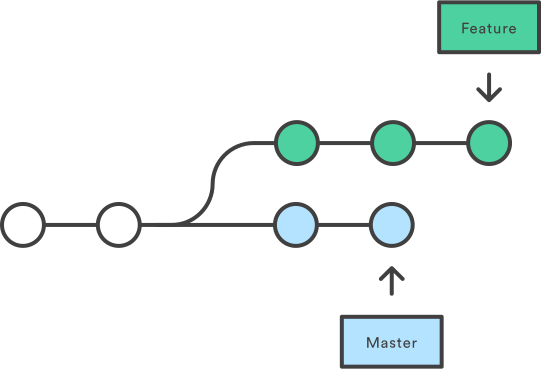
\includegraphics[width=0.59\textwidth]{img/merge/01.png}
\end{frame}

% -------------------------------------------------------------
%
% -------------------------------------------------------------
\begin{frame}{Merging}
  Solution 1:
  \begin{enumerate}
    \item Switch to the Feature branch: \lstinline|git checkout Feature|
    \item Merge: \lstinline|git merge Master|
  \end{enumerate}
  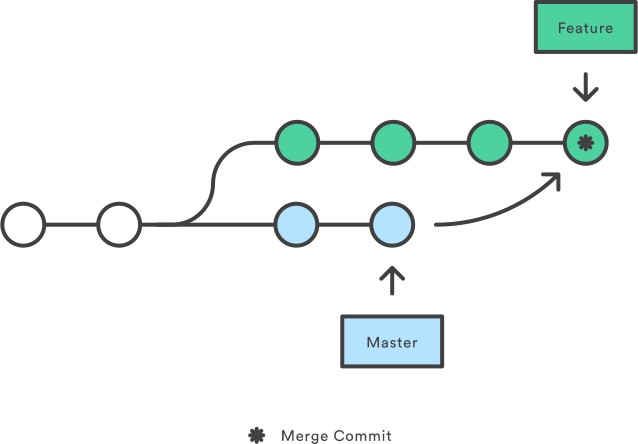
\includegraphics[width=0.695\textwidth]{img/merge/02.png}
\end{frame}

% -------------------------------------------------------------
%
% -------------------------------------------------------------
\begin{frame}{Rebasing}
  Solution 2:
  \begin{enumerate}
    \item Switch to the Feature branch: \lstinline|git checkout Feature|
    \item Rebase: \lstinline|git rebase Master|
  \end{enumerate}
  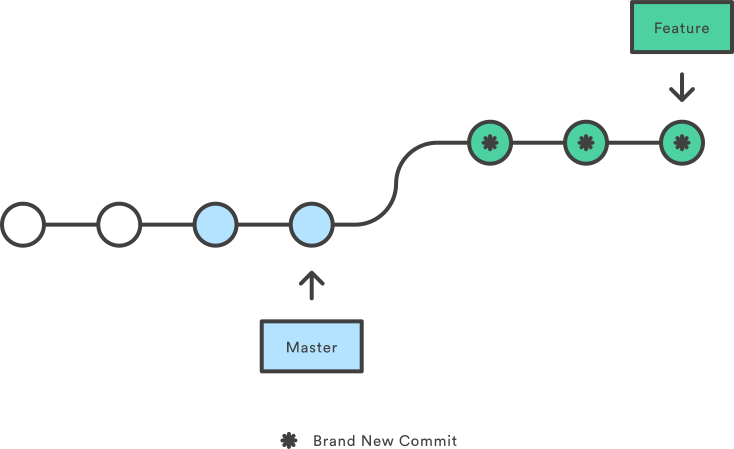
\includegraphics[width=0.8\textwidth]{img/merge/03.png}
  \vspace{-0.06cm}
\end{frame}

% -------------------------------------------------------------
%
% -------------------------------------------------------------
\begin{frame}{Force Pushing}
  Once you have rebased you have a conflict between your local tree and the remote tree.
  \vspace{1cm}
  \begin{columns}
    \begin{column}{0.5\textwidth}
      \centering
      What the remote repository knows:\\
      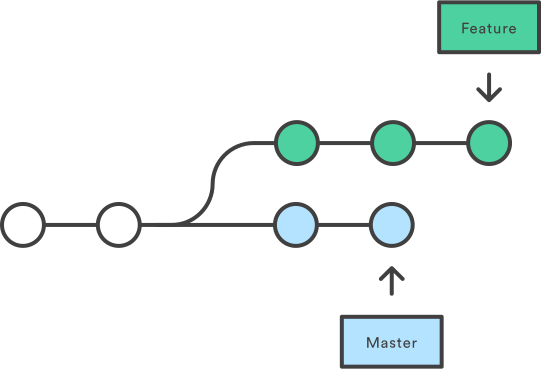
\includegraphics[width=0.59\textwidth]{img/merge/01.png}
    \end{column}
    \begin{column}{0.5\textwidth}
      \centering
      What you have:\\
      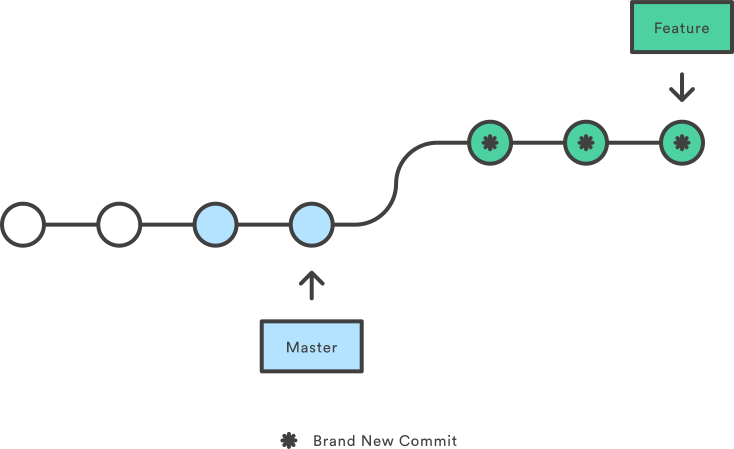
\includegraphics[width=0.8\textwidth]{img/merge/03.png}
      \vspace{-0.5cm}
    \end{column}
  \end{columns}
  \vspace{2.05cm}
\end{frame}

% -------------------------------------------------------------
%
% -------------------------------------------------------------
\begin{frame}{Force Pushing}
  Once you have rebased you have a conflict between your local tree and the remote tree.
  \vspace{1cm}
  \begin{columns}
    \begin{column}{0.5\textwidth}
      \centering
      What the remote repository knows:\\
      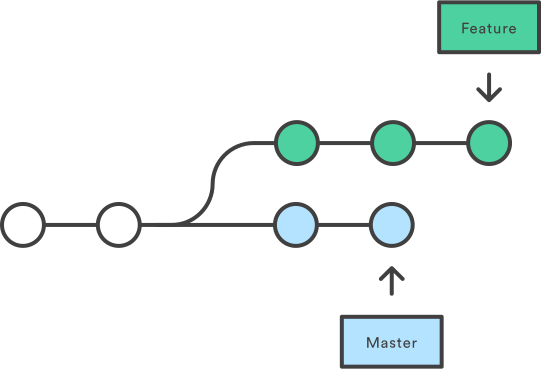
\includegraphics[width=0.59\textwidth]{img/merge/01.png}
    \end{column}
    \begin{column}{0.5\textwidth}
      \centering
      What you have:\\
      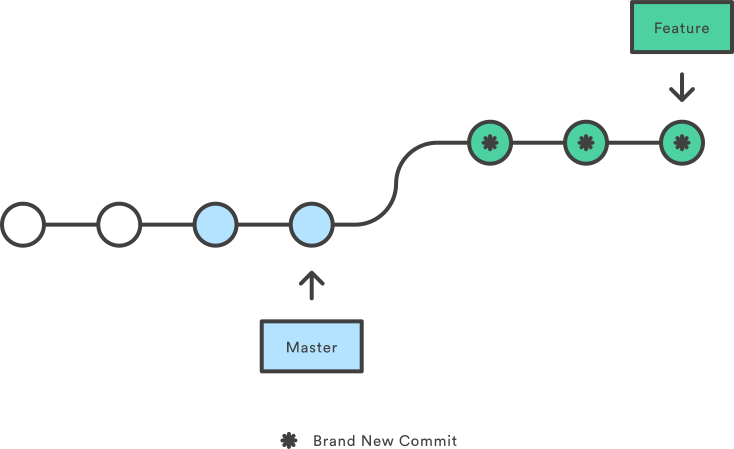
\includegraphics[width=0.8\textwidth]{img/merge/03.png}
      \vspace{-0.5cm}
    \end{column}
  \end{columns}

  \vspace{1cm}
  The solution is a force-push:\\
  \lstinline|git push --force origin Feature|
\end{frame}

% -------------------------------------------------------------
%
% -------------------------------------------------------------
\begin{frame}{Force Pushing}
  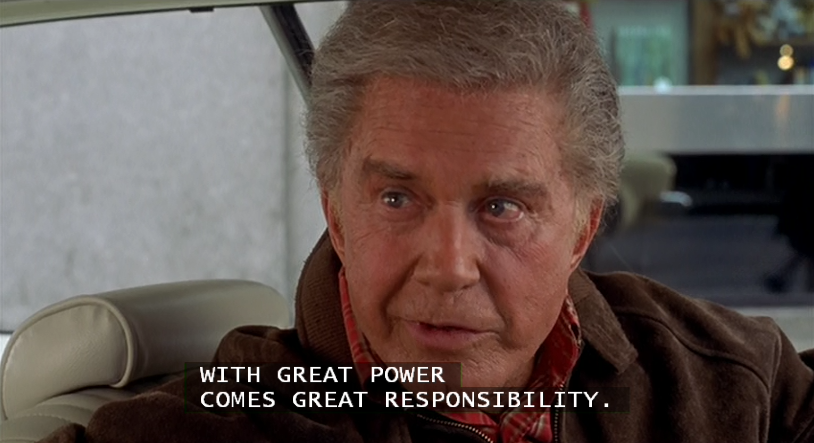
\includegraphics[width=\textwidth]{img/spider-man-2002-uncle-ben-cliff-robertson-great-power.png}

  \alert{\textbf{Force pushing is very dangerous}} and will break everything if not used correctly.
  \begin{itemize}
    \item \alert{\textbf{NEVER force push on Master.}}
    \item \alert{\textbf{ALWAYS specify the repo and the branch.}}
  \end{itemize}
\end{frame}



%%%%%%%%%%%%%%%%%%%%%%%%%%%%%%%%%%%%%%%%%%%%%%%%%%%%%%%
%
%          Conflicts
%
%%%%%%%%%%%%%%%%%%%%%%%%%%%%%%%%%%%%%%%%%%%%%%%%%%%%%%%
\section{Conflicts}

% -------------------------------------------------------------
%
% -------------------------------------------------------------
\begin{frame}[fragile]{Conflicts}
  Conflicts can happen when you do a pull, merge or rebase.

  \lstinline|git merge new_branch_to_merge_later|

  \begin{lstlisting}[basicstyle=\footnotesize\ttfamily]
Auto-merging merge.txt
CONFLICT (content): Merge conflict in merge.txt
Automatic merge failed; fix conflicts and then commit the result.
  \end{lstlisting}
\end{frame}

% -------------------------------------------------------------
%
% -------------------------------------------------------------
\begin{frame}[fragile]{Conflicts}
  \lstinline|git status|

  \begin{lstlisting}[basicstyle=\footnotesize\ttfamily]
On branch master
You have unmerged paths.
(fix conflicts and run "git commit")
(use "git merge --abort" to abort the merge)

Unmerged paths:
(use "git add <file>..." to mark resolution)

both modified:   merge.txt
  \end{lstlisting}
\end{frame}

% -------------------------------------------------------------
%
% -------------------------------------------------------------
\begin{frame}[fragile]{Conflicts}
  \lstinline|cat merge.txt|

  \begin{lstlisting}[basicstyle=\footnotesize\ttfamily]
...
<<<<<<< HEAD
this is some content to mess with
content to append
=======
totally different content to merge later
>>>>>>> new_branch_to_merge_later
...
  \end{lstlisting}
\end{frame}

% -------------------------------------------------------------
%
% -------------------------------------------------------------
\begin{frame}{Conflicts}
  Resolution steps:
  \begin{enumerate}
    \item Edit the file: select the part you like, erase the alternative, save.
    \item \lstinline|git add merge.txt|
    \item \lstinline|git commit -m "Merged and resolved conflict"|
  \end{enumerate}

  In the case of a \lstinline|rebase|, instead of writting a commit message, just do
  \lstinline|git rebase --continue|.

  In both cases, if you are not sure, you can use the \lstinline|--abort| option.
\end{frame}



%%%%%%%%%%%%%%%%%%%%%%%%%%%%%%%%%%%%%%%%%%%%%%%%%%%%%%%
%
%          Reset
%
%%%%%%%%%%%%%%%%%%%%%%%%%%%%%%%%%%%%%%%%%%%%%%%%%%%%%%%
\section{HEAD, Checking out, Reverting \& Resetting}

% -------------------------------------------------------------
%
% -------------------------------------------------------------
\begin{frame}[t]{HEAD \& checkout}
  \vspace{0.5cm}
  The pointer to the current location in Git is called the \textbf{HEAD}.
  It can be used as a reference point.

  E.g. if you want to go back to a previous commit, you can do either:
  \begin{itemize}
    \item \lstinline|git checkout HEAD~2|
    \item \lstinline|git checkout b| where \lstinline|b| is a commit id
  \end{itemize}

  \vspace{0.53cm}
  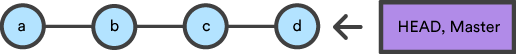
\includegraphics[scale=1.5]{img/undoing/git-sequence-transparent.png}
\end{frame}

% -------------------------------------------------------------
%
% -------------------------------------------------------------
\begin{frame}[t]{HEAD \& checkout}
  \vspace{0.5cm}
  The pointer to the current location in Git is called the \textbf{HEAD}.
  It can be used as a reference point.

  E.g. if you want to go back to a previous commit, you can do either:
  \begin{itemize}
    \item \lstinline|git checkout HEAD~2|
    \item \lstinline|git checkout b| where \lstinline|b| is a commit id
  \end{itemize}

  \vspace{0.5cm}
  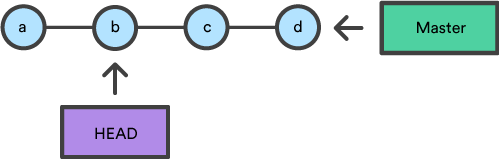
\includegraphics[scale=1.5]{img/undoing/2497537634-git-checkout-transparent.png}

  From there you can start working on a new branch: \lstinline|git checkout -b Foo|
\end{frame}

% -------------------------------------------------------------
%
% -------------------------------------------------------------
\begin{frame}{Changing the commit message}
  You can rewrite the message of the last commit with:\\
  \lstinline|git commit --amend|

  \vspace{0.5cm}
  \only<1>{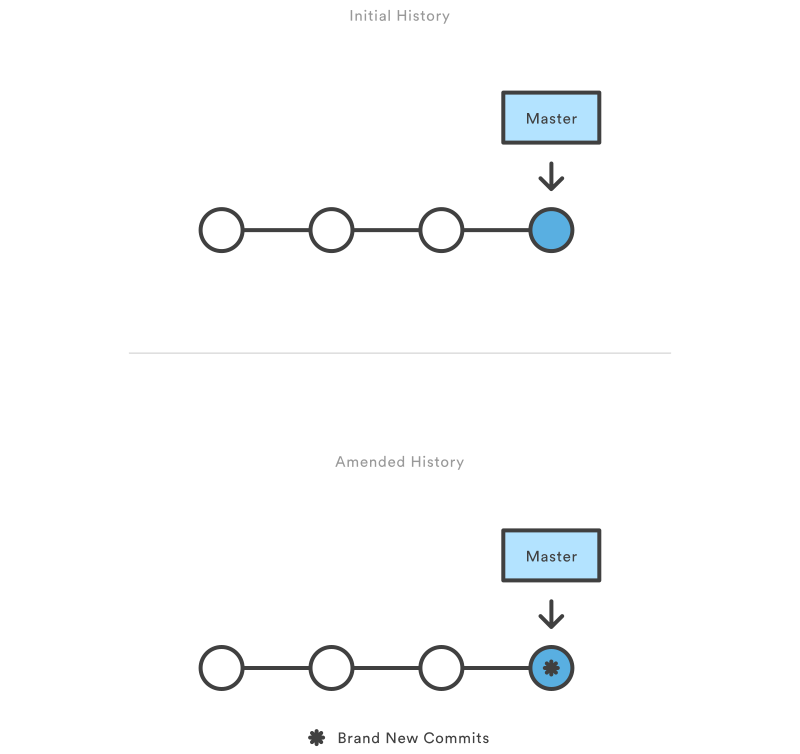
\includegraphics[width=0.5\textwidth]{img/rewriting/01.png}}
  \only<2>{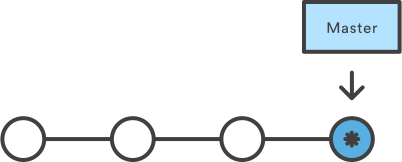
\includegraphics[width=0.5\textwidth]{img/rewriting/02.png}}
\end{frame}

% -------------------------------------------------------------
%
% -------------------------------------------------------------
\begin{frame}{Reverting}
  If you want to undo the last commit: \lstinline|git revert HEAD|\\
  This will \textbf{create} a new commit which reverts the lastest changes.

  \vspace{0.5cm}
  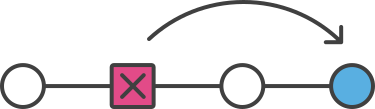
\includegraphics[width=0.5\textwidth]{img/undoing/02.png}

  If you want to undo changes from an older commit you can also do:
  \lstinline|git revert commit_id| e.g. \lstinline|git revert a1e8bf5| or \lstinline|git revert HEAD~1|
\end{frame}

% -------------------------------------------------------------
%
% -------------------------------------------------------------
\begin{frame}{Resetting}
  \lstinline|git reset --... commit_id| comes with 2 main options:
  \begin{itemize}
    \item \lstinline|--soft|: keep the files as is but reset the pointer to \lstinline|commit_id|.
    \item \lstinline|--hard|: reset the files to the pointer \lstinline|commit_id|.
  \end{itemize}

  \vspace{0.5cm}
  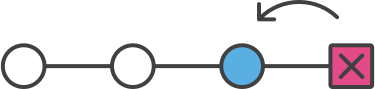
\includegraphics[width=0.5\textwidth]{img/undoing/03.png}
\end{frame}

% -------------------------------------------------------------
%
% -------------------------------------------------------------
\begin{frame}{Reset tricks}
  \begin{itemize}
    \item \lstinline|git reset --hard HEAD|: remove all the changes made from the HEAD\\~\\
    \item \lstinline|git reset --soft HEAD~4|: go back and forget 4 commits but leave the files as-is. Useful if you want to squash your history.\\~\\
    \item \lstinline|git reset --hard commit_id|: set the repository as it was in \lstinline|commit_id|
  \end{itemize}
\end{frame}



\section{Stage, Diff, Stash, Clean}

% -------------------------------------------------------------
%
% -------------------------------------------------------------
\begin{frame}{Staged files and diff}
  Files have 4 states:
  \begin{itemize}
    \item Committed
    \item Staged
    \item Unstaged
    \item Untracked
  \end{itemize}
  Staged files contain changes that are recorded by Git but not committed yet.

  \lstinline|git diff| will show the diff between staged/committed and unstaged files.
\end{frame}

% -------------------------------------------------------------
%
% -------------------------------------------------------------
\begin{frame}{Stash}
  \lstinline|git stash| comes with 4 main option:
  \begin{itemize}
    \item \lstinline|push|: (optional) save your local modifications and revert to HEAD.
    \item \lstinline|pop|: apply the modifications on top of the current working tree state.
    \item \lstinline|list|
    \item \lstinline|clear|
  \end{itemize}

  \vspace{0.5cm}
  During a \lstinline|git stash ; git stash pop|, all modifications are unstaged.
\end{frame}

% -------------------------------------------------------------
%
% -------------------------------------------------------------
\begin{frame}{Clean}
  You modified a lot of files, you have a lot of untracked files, your repository is dirty?
  Don't worry, \lstinline|git clean| is here for you!
  \begin{itemize}
    \item \lstinline|git clean -nd|: list the files to be removed
    \item \lstinline|git clean -fd|: remove recursively (\lstinline|-d|) untracked files
    \item \lstinline|git clean -fxd|: remove recursively untracked and ignored (\lstinline|-x|) files
  \end{itemize}

  \vspace{0.5cm}
  By default \lstinline|git clean| will do nothing, it requires either:
  \begin{itemize}
    \item \lstinline|-n| for a dry-run.
    \item \lstinline|-f| for force
  \end{itemize}
\end{frame}



%%%%%%%%%%%%%%%%%%%%%%%%%%%%%%%%%%%%%%%%%%%%%%%%%%%%%%%
%
%          Bonus
%
%%%%%%%%%%%%%%%%%%%%%%%%%%%%%%%%%%%%%%%%%%%%%%%%%%%%%%%
\section{Workflow: All on Master\\(classic academia)}

% -------------------------------------------------------------
%
% -------------------------------------------------------------
\begin{frame}[fragile,t]{All on Master}
  \begin{center}
    \includegraphics<1>[width=0.5\textwidth]{img/Workflow/01.png}
    \includegraphics<2>[width=0.5\textwidth]{img/Workflow/02.png}
    \includegraphics<3>[width=0.5\textwidth]{img/Workflow/03.png}
    \includegraphics<4>[width=0.5\textwidth]{img/Workflow/04.png}
    \includegraphics<5>[width=0.5\textwidth]{img/Workflow/05.png}
    \includegraphics<6>[width=0.8\textwidth]{img/Workflow/06.png}
    \includegraphics<7-9>[width=0.7\textwidth]{img/Workflow/08.png}
    \includegraphics<10>[width=0.5\textwidth]{img/Workflow/09.png}

    \only<1>{John works on his feature}
    \only<2>{Mary works on her feature}
    \only<3>{
    John publishes his feature\\
    \lstinline|git push origin master|}
    \only<4>{
    Mary tries to publish her feature\\
    \lstinline|git push origin master|}
    \only<5>{
    Mary rebases on top of John’s commit(s)\\
    \lstinline|git pull --rebase origin master|}
    \only<6>{Expected new tree (Mary's POV).}
    \only<7>{But there is a conflict...}
    \only<8>{\lstinline|git status|}
    \only<9>{Mary edits \texttt{<some-file>}}
    \only<10>{
    Mary successfully publishes her feature\\
    \lstinline|git push origin master|}
  \end{center}

  \begin{onlyenv}<4>
    \begin{lstlisting}[basicstyle=\scriptsize\ttfamily]
error: failed to push some refs to '/path/to/repo.git'
hint: Updates were rejected because the tip of your current branch is behind
hint: its remote counterpart. Merge the remote changes (e.g. 'git pull')
hint: before pushing again.
    \end{lstlisting}
  \end{onlyenv}

  \begin{onlyenv}<7>
    \begin{lstlisting}[basicstyle=\scriptsize\ttfamily]
CONFLICT (content): Merge conflict in <some-file>
    \end{lstlisting}
  \end{onlyenv}

  \begin{onlyenv}<8>
    \begin{lstlisting}[basicstyle=\scriptsize\ttfamily]
# Unmerged paths:
# (use "git reset HEAD <some-file>..." to unstage)
# (use "git add/rm <some-file>..." as appropriate to mark resolution)
#
# both modified: <some-file>
    \end{lstlisting}
  \end{onlyenv}

  \begin{onlyenv}<9>
    \begin{lstlisting}[basicstyle=\scriptsize\ttfamily]
git add <some-file>
git rebase --continue
    \end{lstlisting}
  \end{onlyenv}
\end{frame}



%%%%%%%%%%%%%%%%%%%%%%%%%%%%%%%%%%%%%%%%%%%%%%%%%%%%%%%
%
%          Branch flow
%
%%%%%%%%%%%%%%%%%%%%%%%%%%%%%%%%%%%%%%%%%%%%%%%%%%%%%%%
\section{Workflow: Branch Workflow}

% -------------------------------------------------------------
%
% -------------------------------------------------------------
\begin{frame}[fragile,t]{Using Branches and Pull Requests}
  \begin{center}
    \includegraphics<1>[width=0.8\textwidth]{img/Workflow2/01.png}
    \includegraphics<2>[width=0.5\textwidth]{img/Workflow2/02.png}
    \includegraphics<3>[width=0.5\textwidth]{img/Workflow2/03.png}
    \includegraphics<4>[width=0.5\textwidth]{img/Workflow2/04.png}
    \includegraphics<5>[width=0.5\textwidth]{img/Workflow2/05.png}
    \includegraphics<6>[width=0.8\textwidth]{img/Workflow2/06.png}
  \end{center}

  \only<1>{Mary begins a new feature\\
    \lstinline|git checkout -b marys-feature master|\\
    \lstinline|git status|\\
    \lstinline|git add <some-file>|\\
    \lstinline|git commit|
  }
  \only<2>{Mary goes to lunch\\
  \lstinline|git push -u origin marys-feature|}
  \only<3>{
    Mary finishes her feature\\
    \lstinline|git push|
  }
  \only<4>{Bill receives the Pull Request, reviews and [requests changes/ comments/approves]}
  \only<5>{Mary makes the changes}
  \only<6>{
    Mary publishes her feature\\
    \lstinline|git checkout master|\\
    \lstinline|git pull|\\
    \lstinline|git merge marys-feature|\\
    \lstinline|git push|
  }
\end{frame}



%%%%%%%%%%%%%%%%%%%%%%%%%%%%%%%%%%%%%%%%%%%%%%%%%%%%%%%
%
%          Gitflow
%
%%%%%%%%%%%%%%%%%%%%%%%%%%%%%%%%%%%%%%%%%%%%%%%%%%%%%%%
\section{Gitflow Workflow}

% -------------------------------------------------------------
%
% -------------------------------------------------------------
\begin{frame}[t]{Gitflow Workflow}
  \begin{center}
    \only<1>{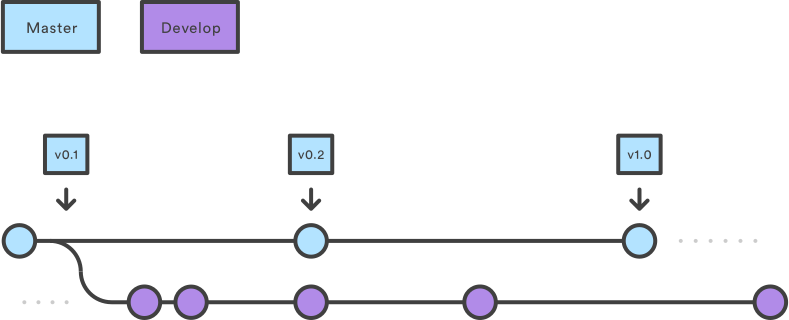
\includegraphics[width=0.8\textwidth]{img/Workflow3/01.png}}
    \only<2>{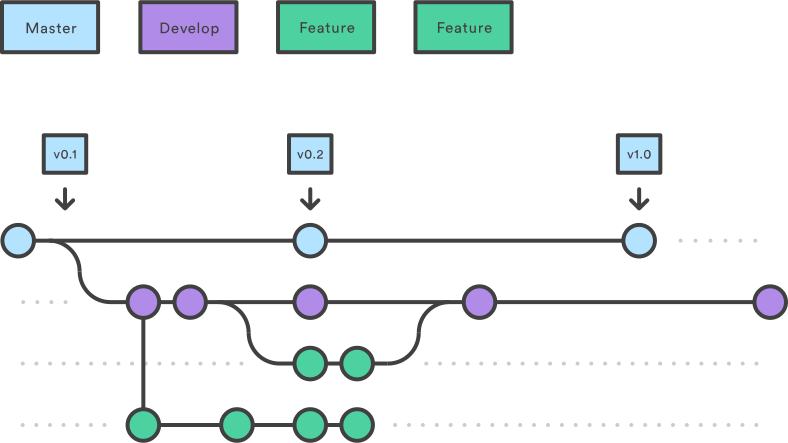
\includegraphics[width=0.8\textwidth]{img/Workflow3/02.png}}
    \only<3>{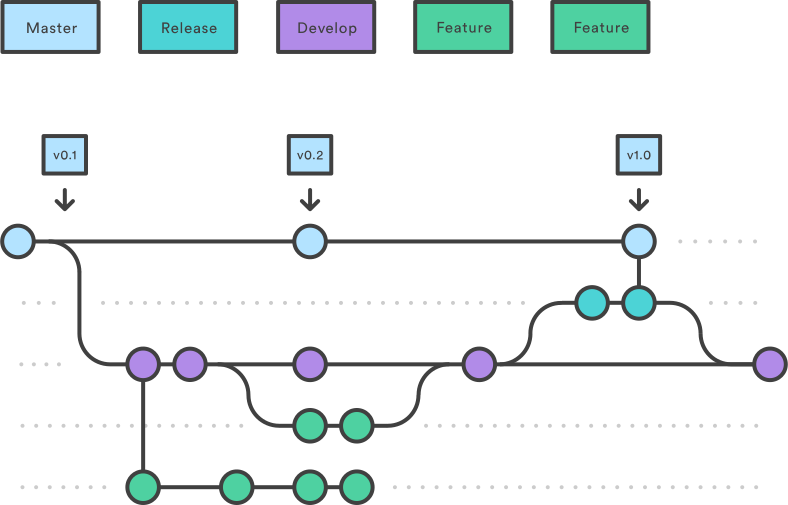
\includegraphics[width=0.8\textwidth]{img/Workflow3/03.png}}
    \only<4>{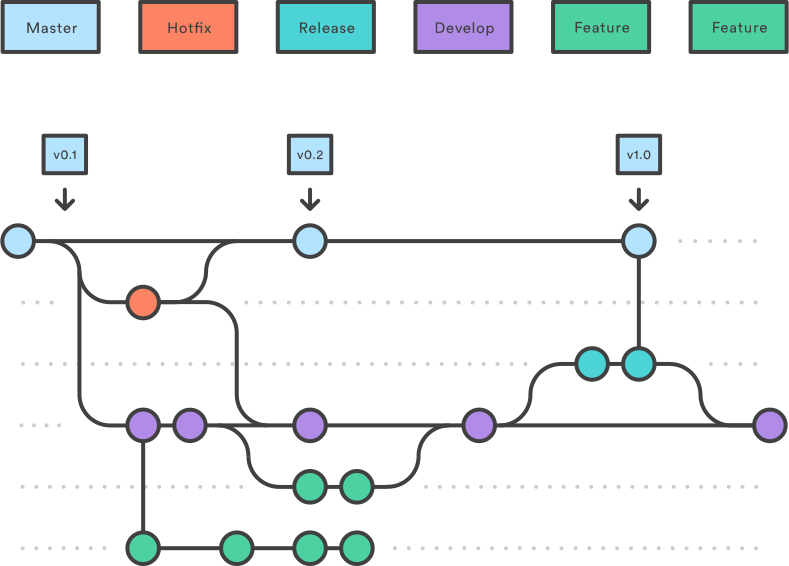
\includegraphics[width=0.8\textwidth]{img/Workflow3/04.png}}

    \begin{onlyenv}<1>
      Develop and Master Branches.
      \begin{itemize}
        \item Master branch only contains the minor and major versions.\\
        $\implies$ e.g.\,\emph{Debian Stable}
        \item Develop branch contains all the intermediate modifications.\\
        $\implies$ e.g.\,\emph{Debian Unstable}
      \end{itemize}
    \end{onlyenv}
    \begin{onlyenv}<2>
      \begin{itemize}
        \item Features are developped as branches of the Develop branch.\\
        $\implies$ e.g.\,\emph{Debian Experimental}
      \end{itemize}
    \end{onlyenv}
    \begin{onlyenv}<3>
      \begin{itemize}
        \item A Release branch contains the "frozen" features.\\
        $\implies$ e.g.\,\emph{Debian Testing}
      \end{itemize}
    \end{onlyenv}
    \begin{onlyenv}<4>
      \begin{itemize}
        \item if an issue is detected in master a hotfix branch is created from master
      \end{itemize}
    \end{onlyenv}
  \end{center}
\end{frame}



%%%%%%%%%%%%%%%%%%%%%%%%%%%%%%%%%%%%%%%%%%%%%%%%%%%%%%%
%
%          Bonus
%
%%%%%%%%%%%%%%%%%%%%%%%%%%%%%%%%%%%%%%%%%%%%%%%%%%%%%%%
\section{Bonus}


\begin{frame}[fragile]{bonus}
  In your \;\texttt{\textapprox/.bashrc} or \;\texttt{\textapprox/.zshrc}:

  \lstinline|alias gtree='git log --oneline --decorate --all --graph'|

  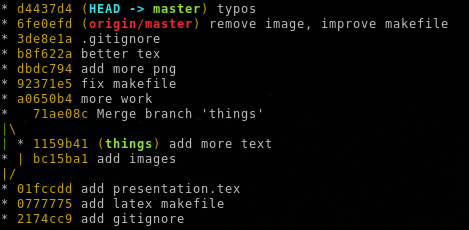
\includegraphics[width=0.5\textwidth]{img/gtree.png}
\end{frame}


\begin{frame}[standout]
Thank you.
\end{frame}

\end{document}
